\section{Experimentación Y Resultados}

A continuación expondremos los resultados obtenidos por cada algoritmo para distintas imágenes. El objetivo será posteriormente hacer análisis de calidad subjetiva (es decir que vemos a simple vista), objetiva y tiempo de computos. Para, como dijimos en un principio, determinar ventajas y desventajas de cada uno de ellos.

\subsection{Colores}

Se nos ocurrió que podría ser interesante chequear los comportamientos de estos procedimientos en una imagen con muchos bordes ya que estos, en algoritmos como el directional, son factores importantes y potencialmente conflictivos.

\begin{figure}[!htb]
\begin{center}
       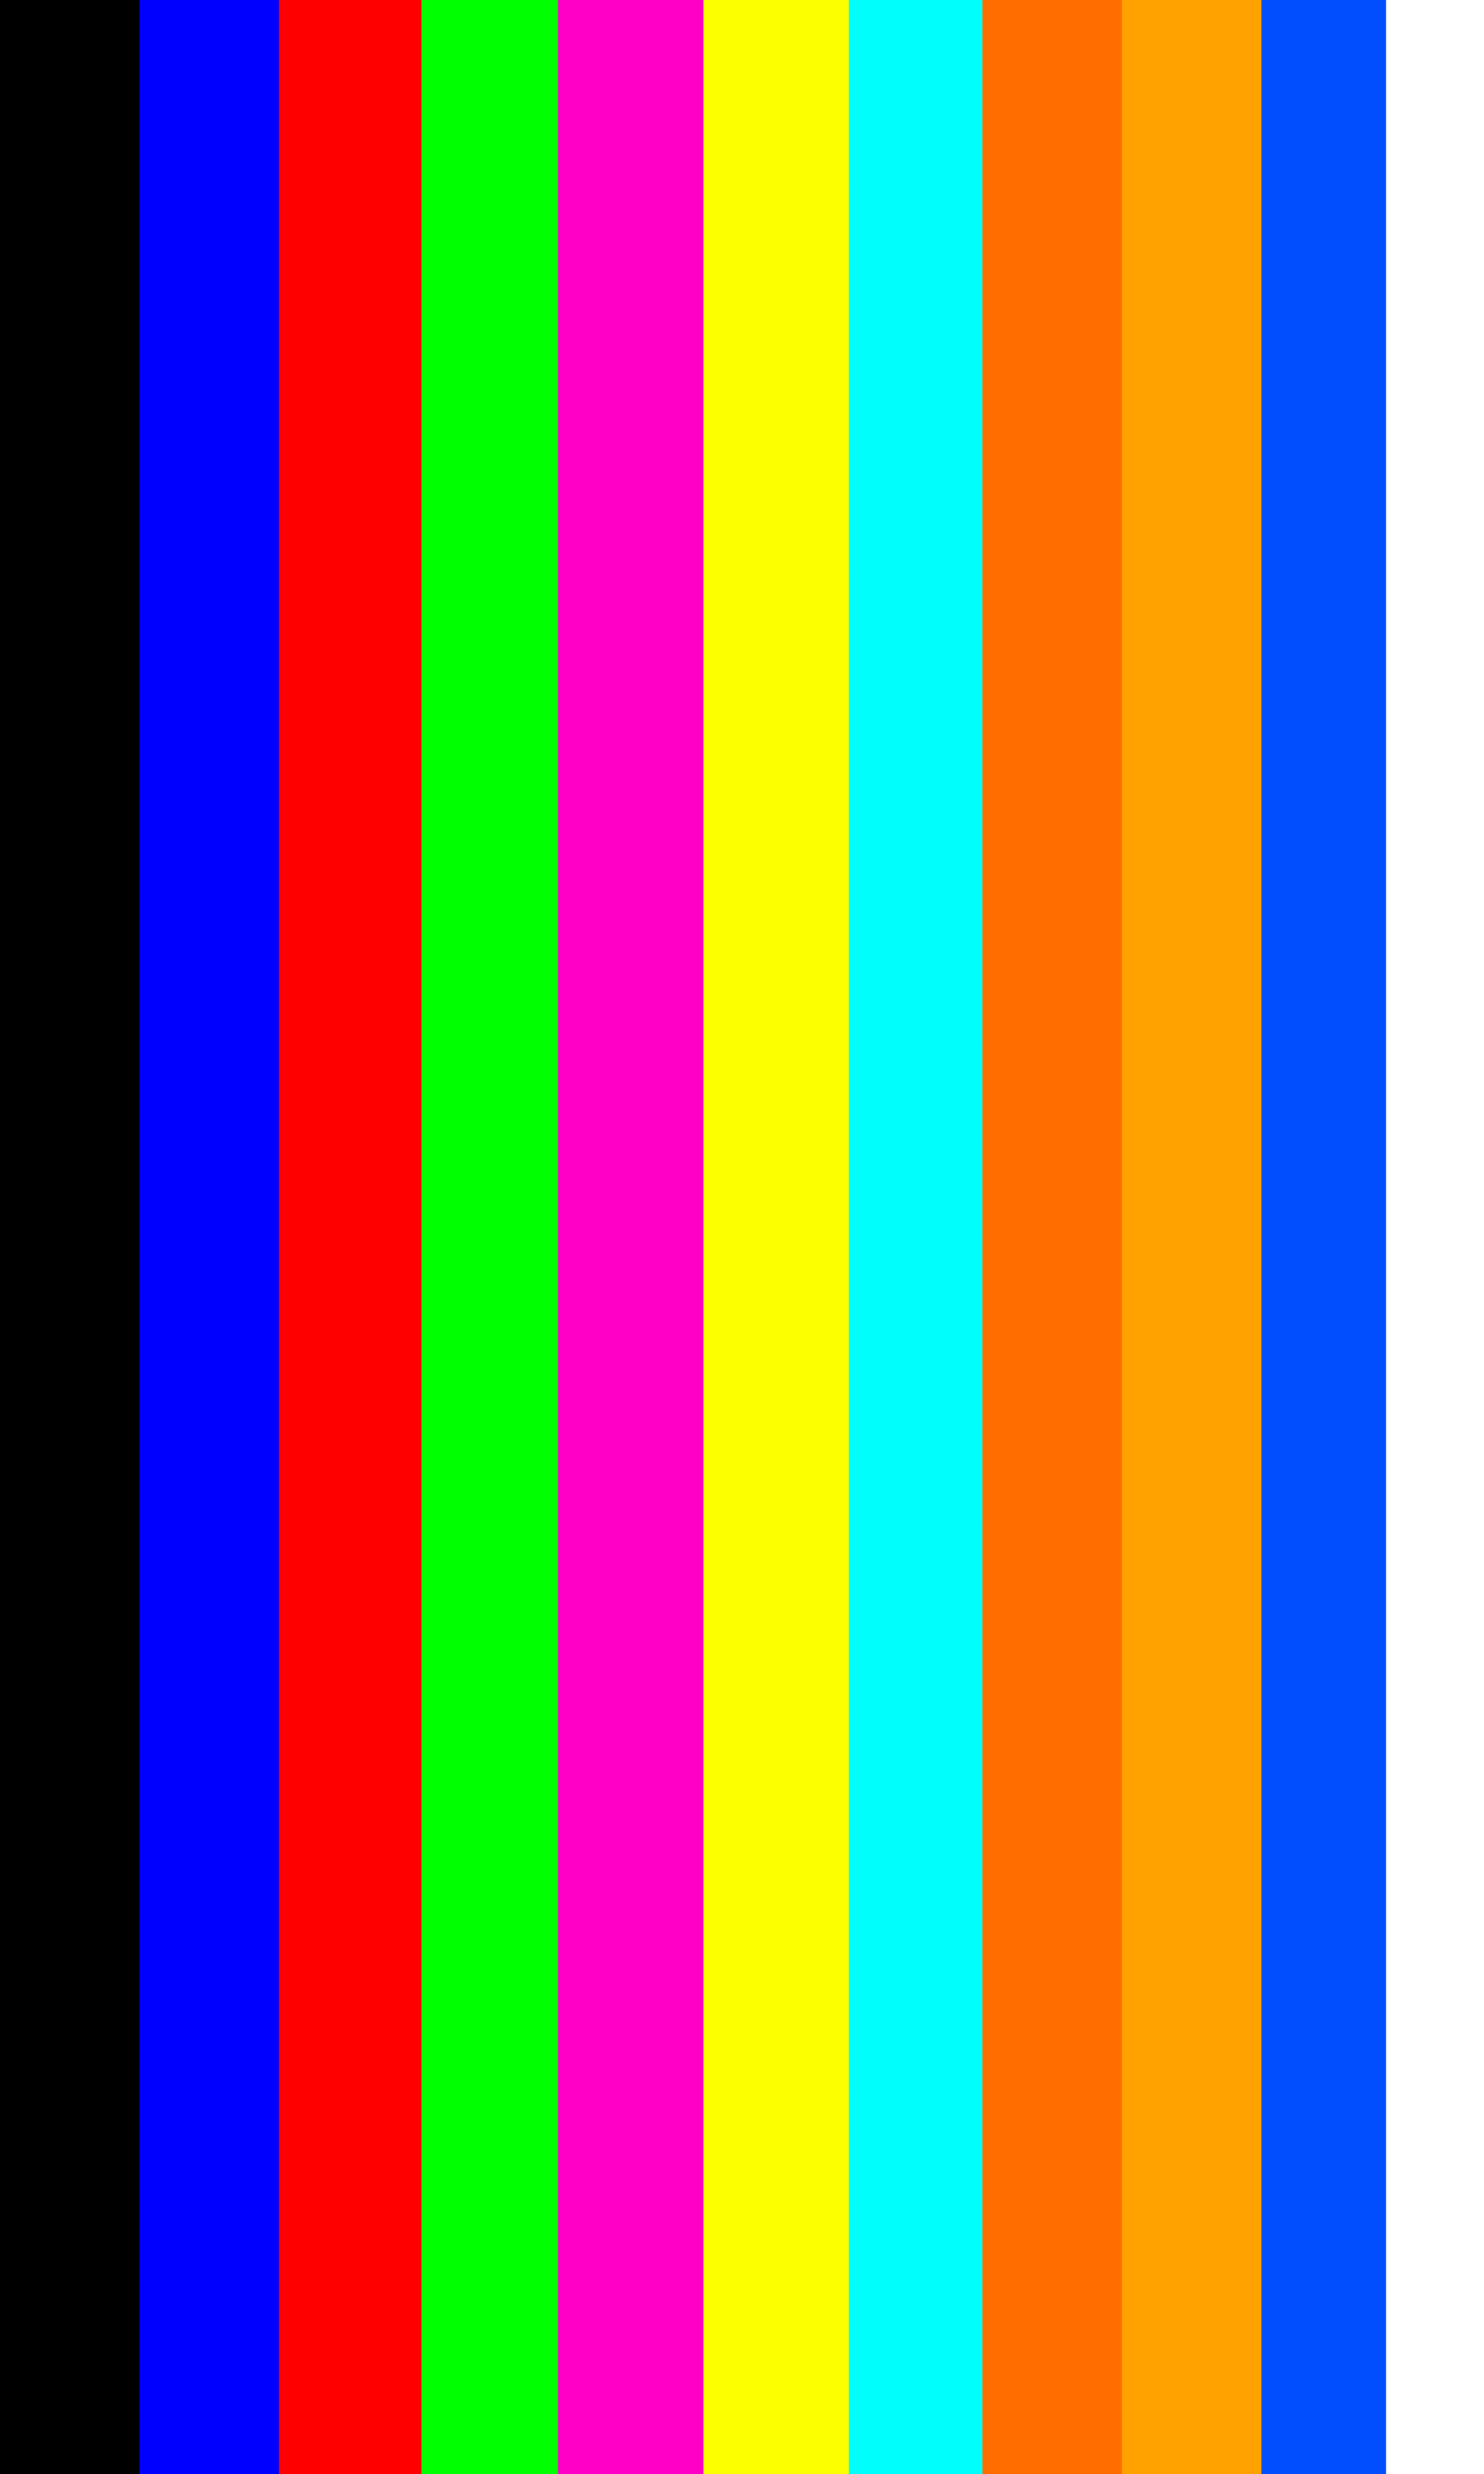
\includegraphics[scale=0.5]{imagenes/colores.png}
       \caption{Original }
  \end{center}
\end{figure}
\begin{figure}[!htb]
\begin{center}
        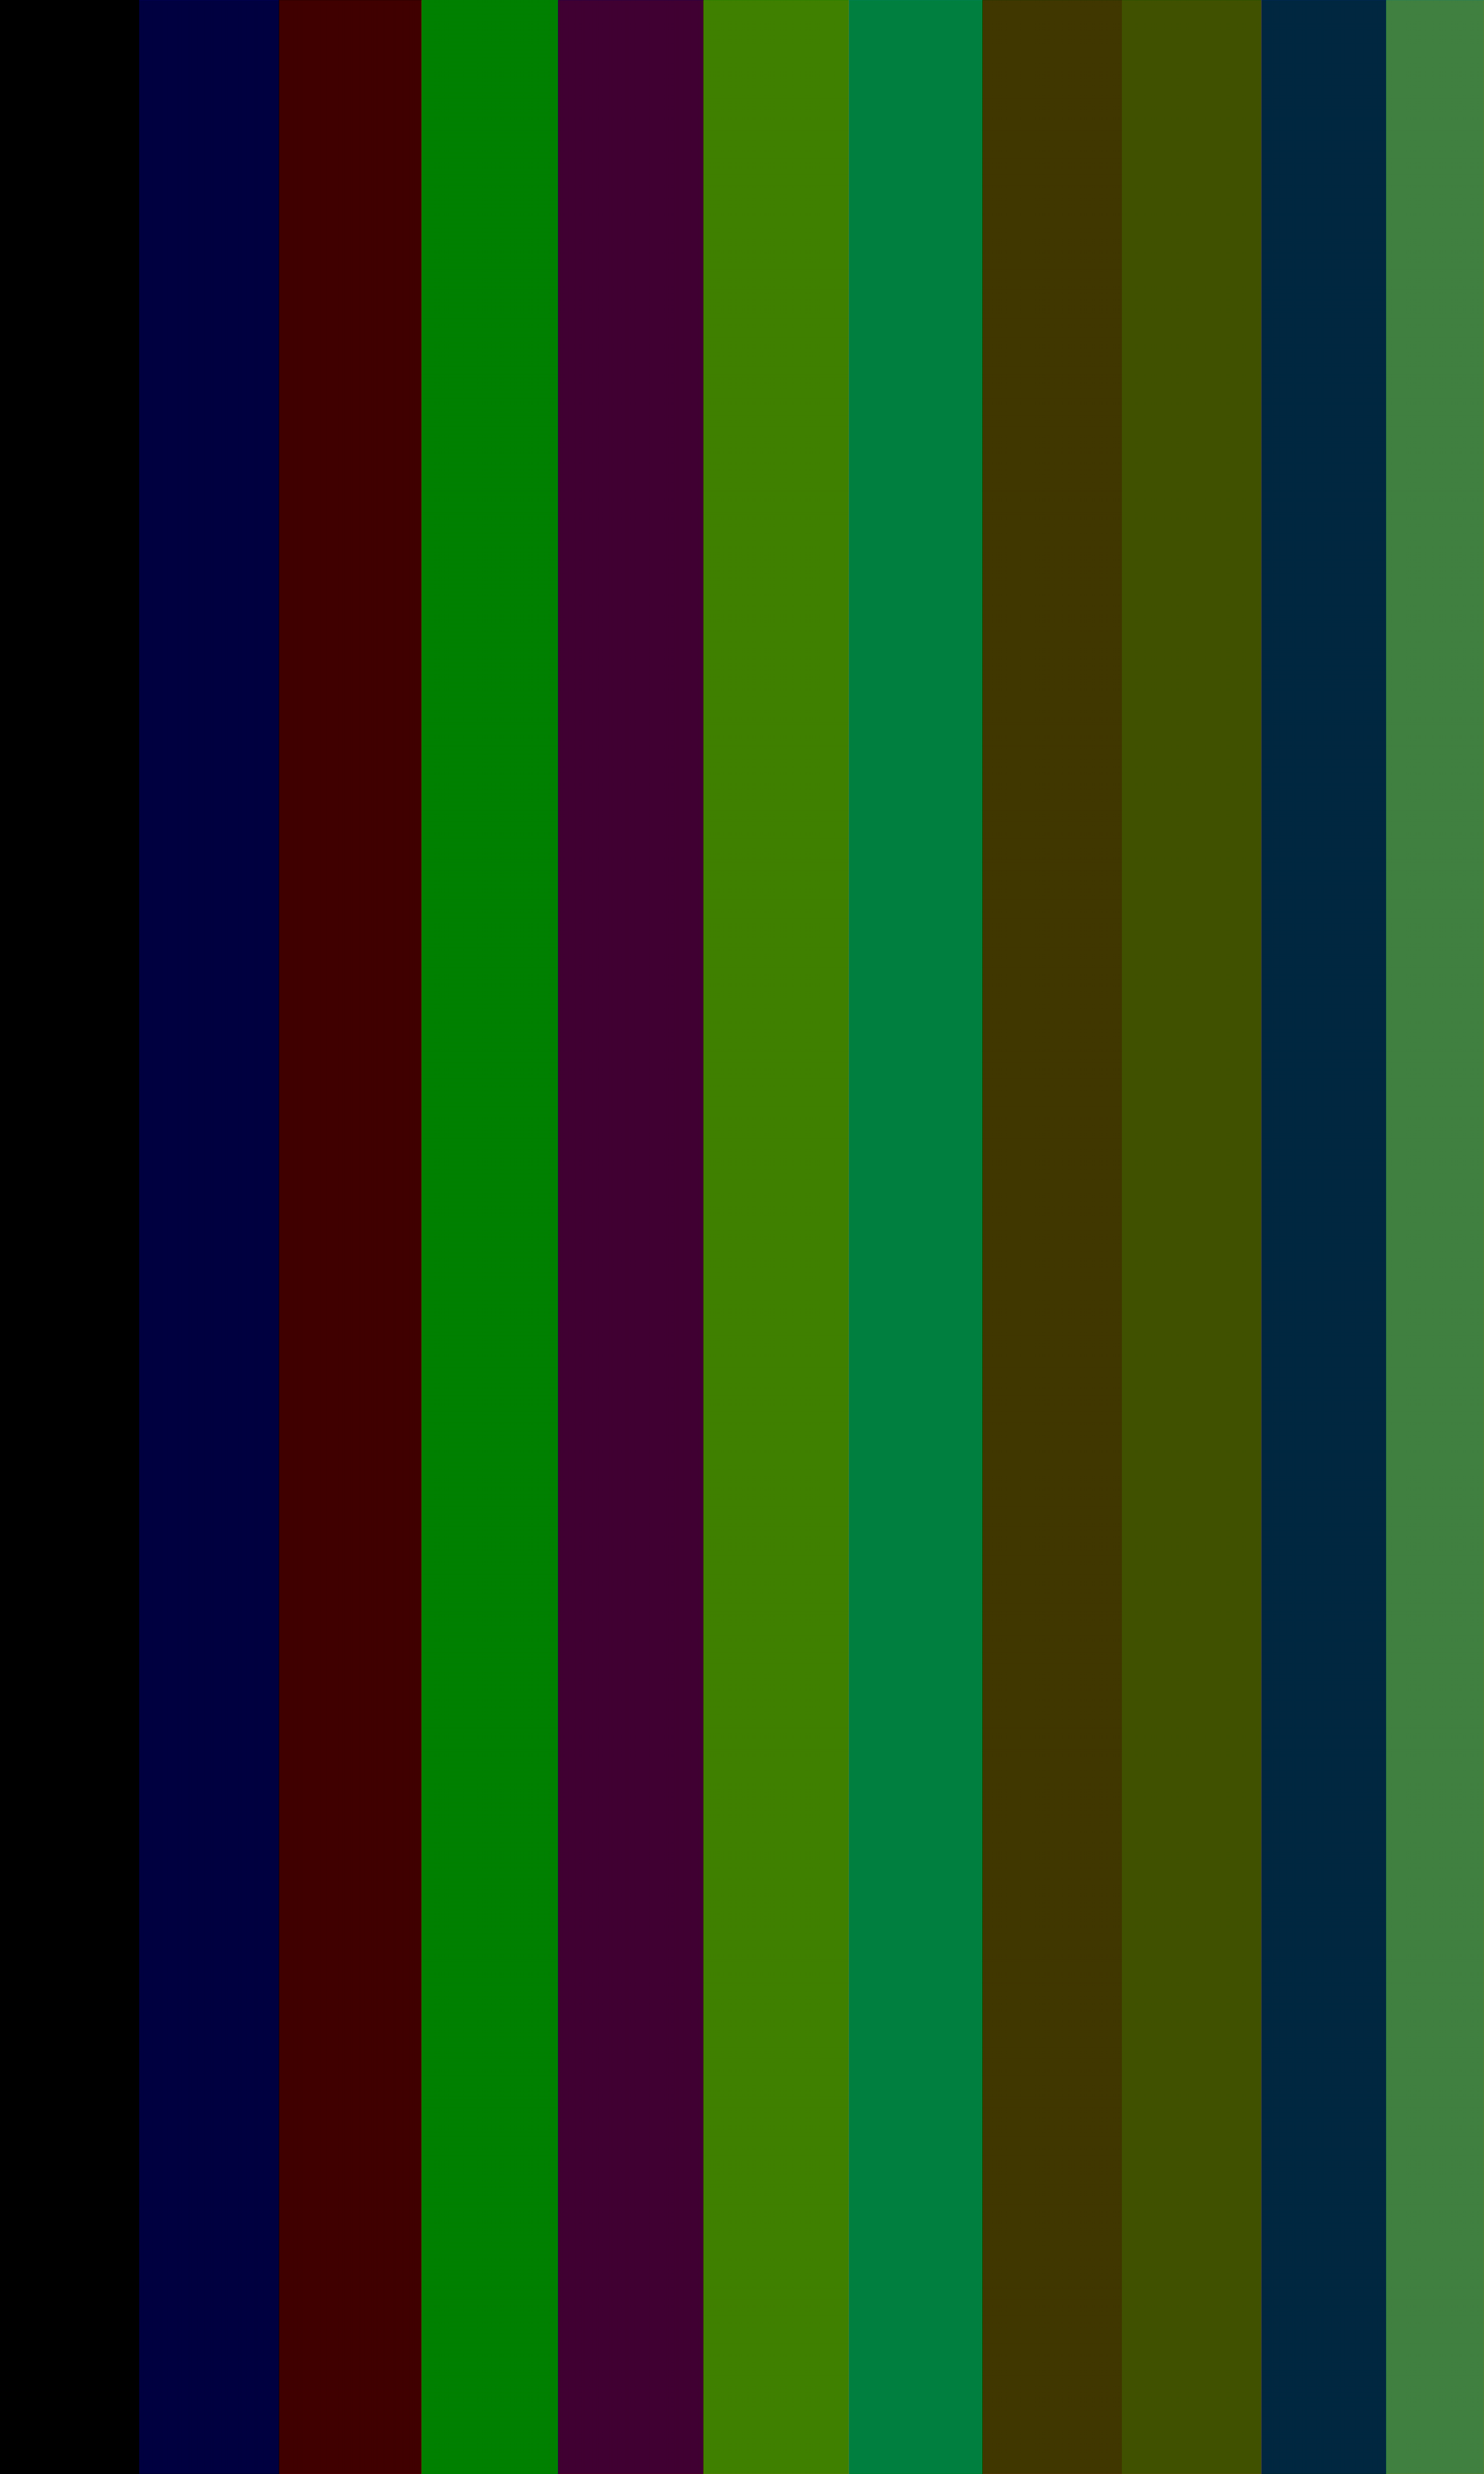
\includegraphics[scale=0.5]{imagenes/colores_bayer.png}
       \caption{Bayerizada}
       \end{center}
\end{figure}

\begin{figure}[!htb]
\begin{center}
    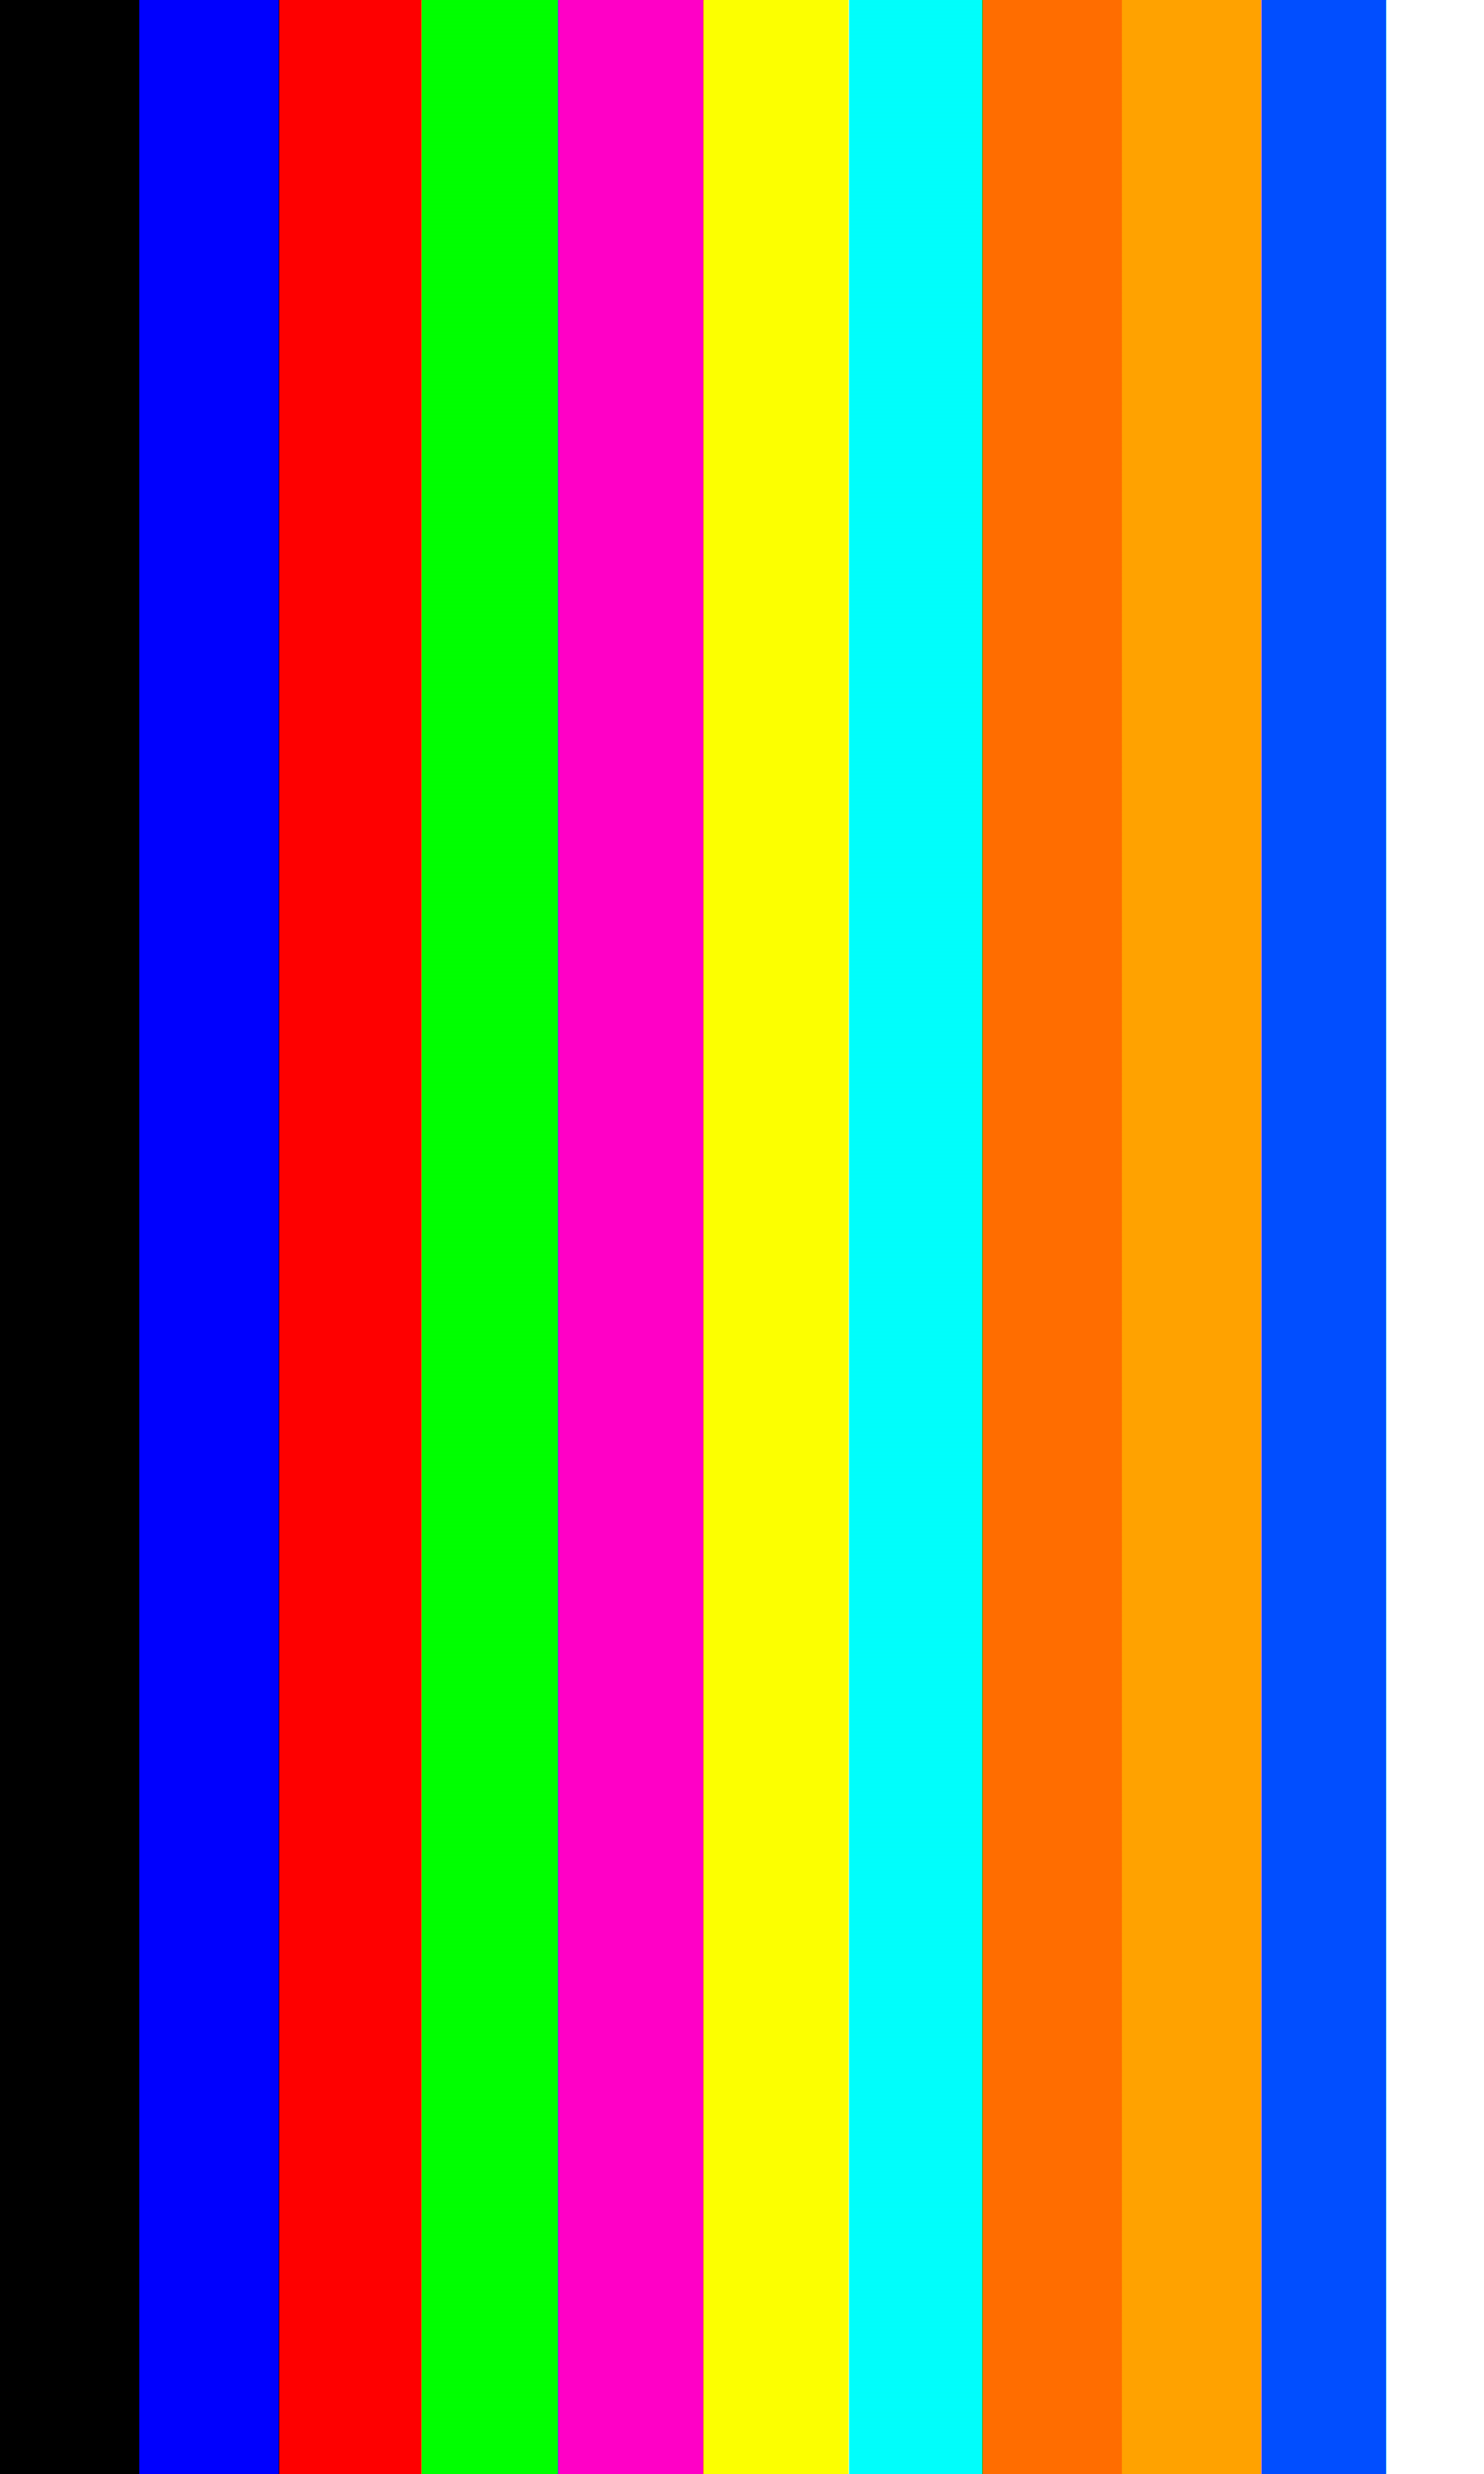
\includegraphics[scale=0.5]{imagenes/colores_demosicing_bilineal.png}
    \caption{Bilineal }
  \end{center}
\end{figure}
\begin{figure}[!htb]
\begin{center}
    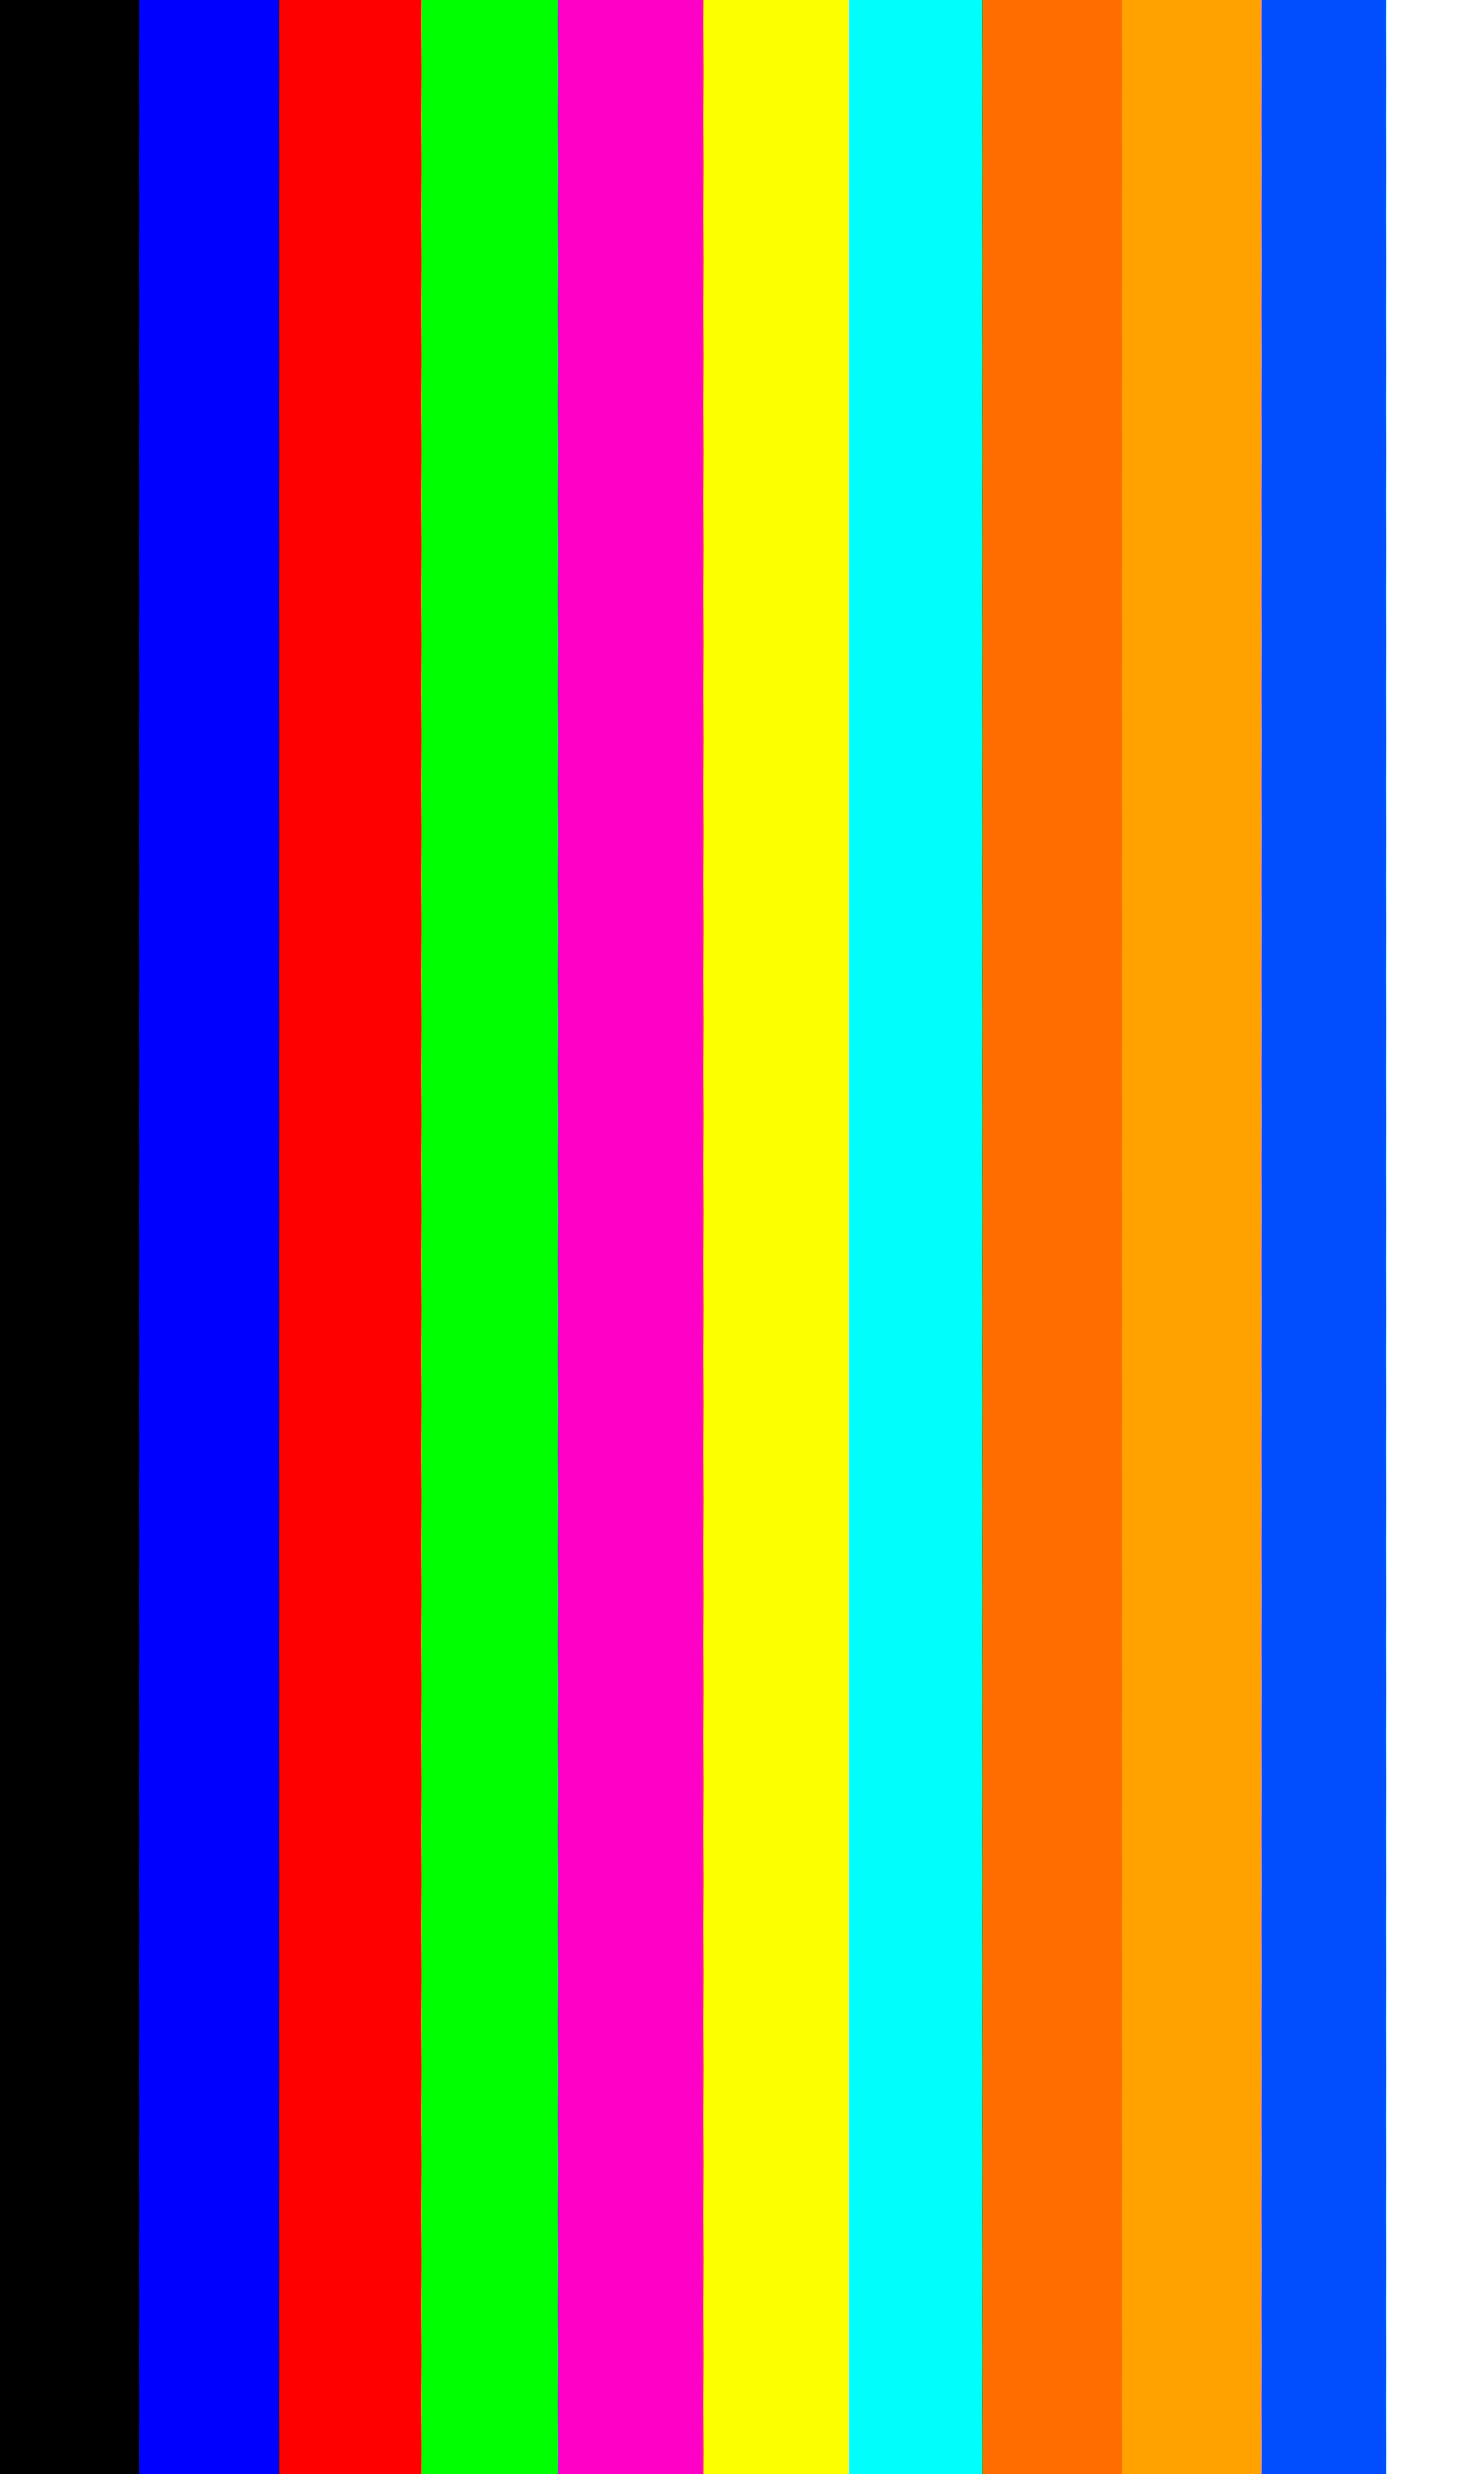
\includegraphics[scale=0.5]{imagenes/colores_demosicing_quality.png}
    \caption{High Quality}
    \end{center}
\end{figure}
\begin{figure}[!htb]
\begin{center}
    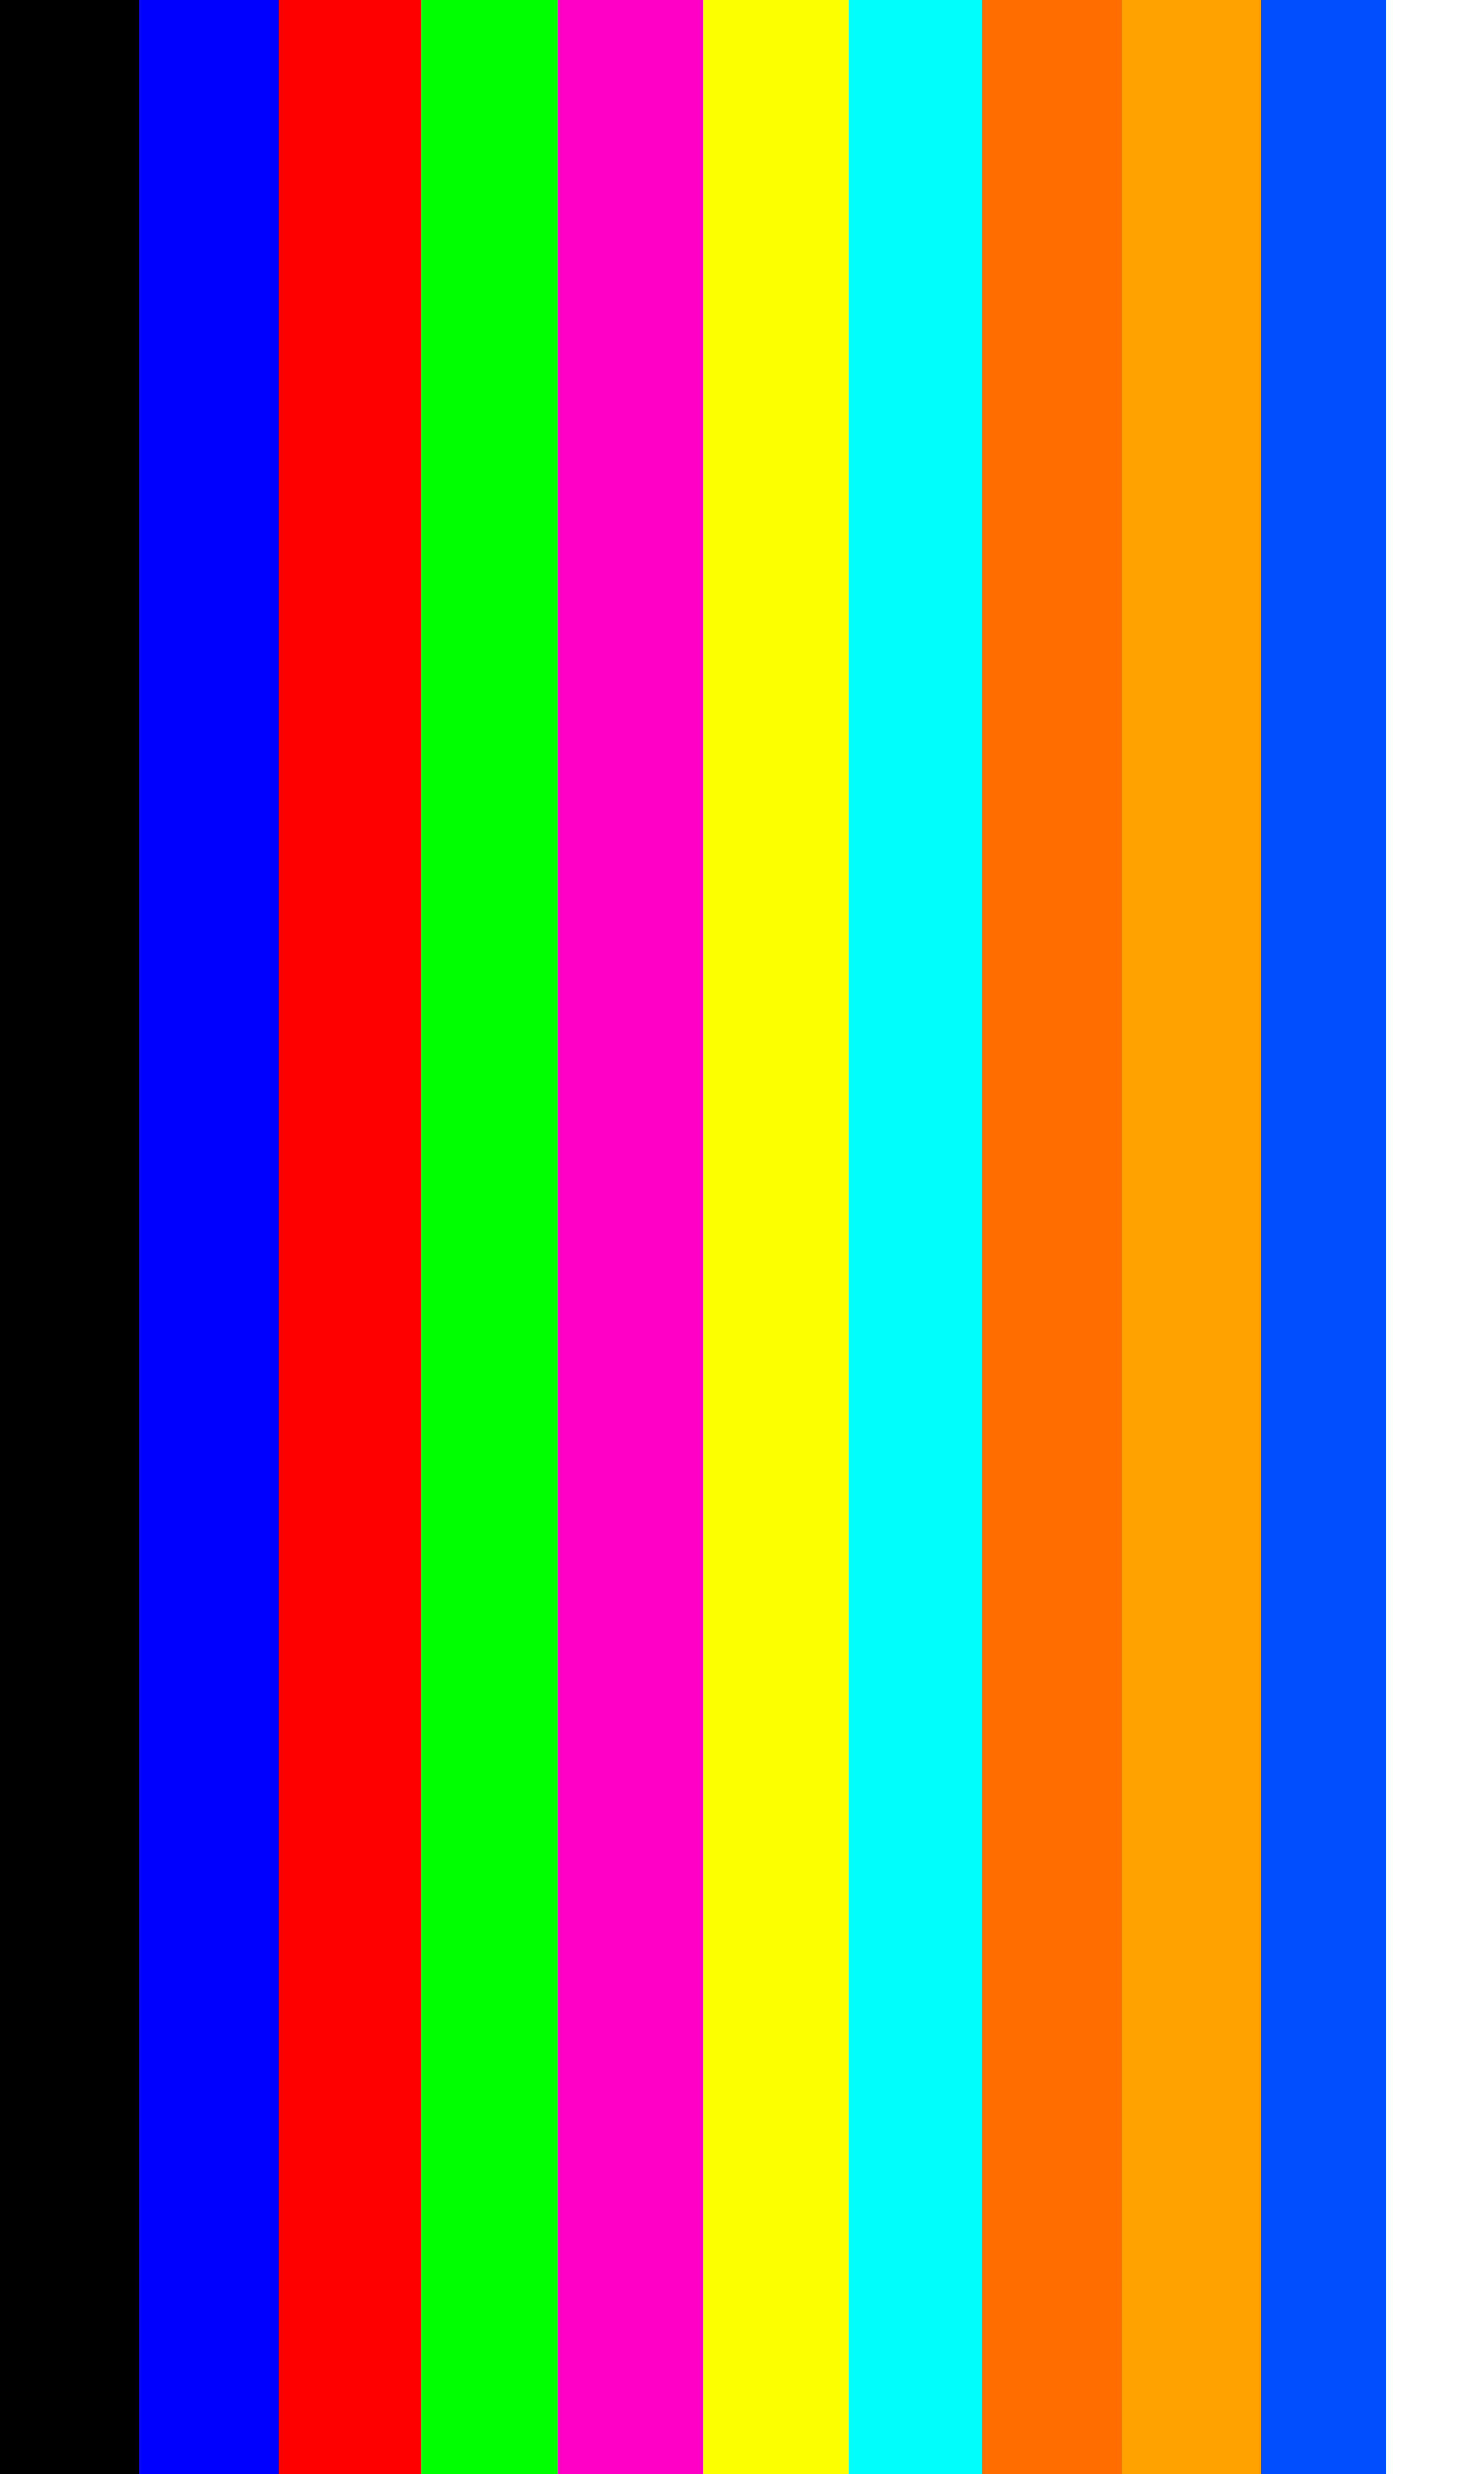
\includegraphics[scale=0.5]{imagenes/colores_demosicing_spline.png}
    \caption{Directional}
    \end{center}
\end{figure}
\begin{figure}[!htb]
\begin{center}
    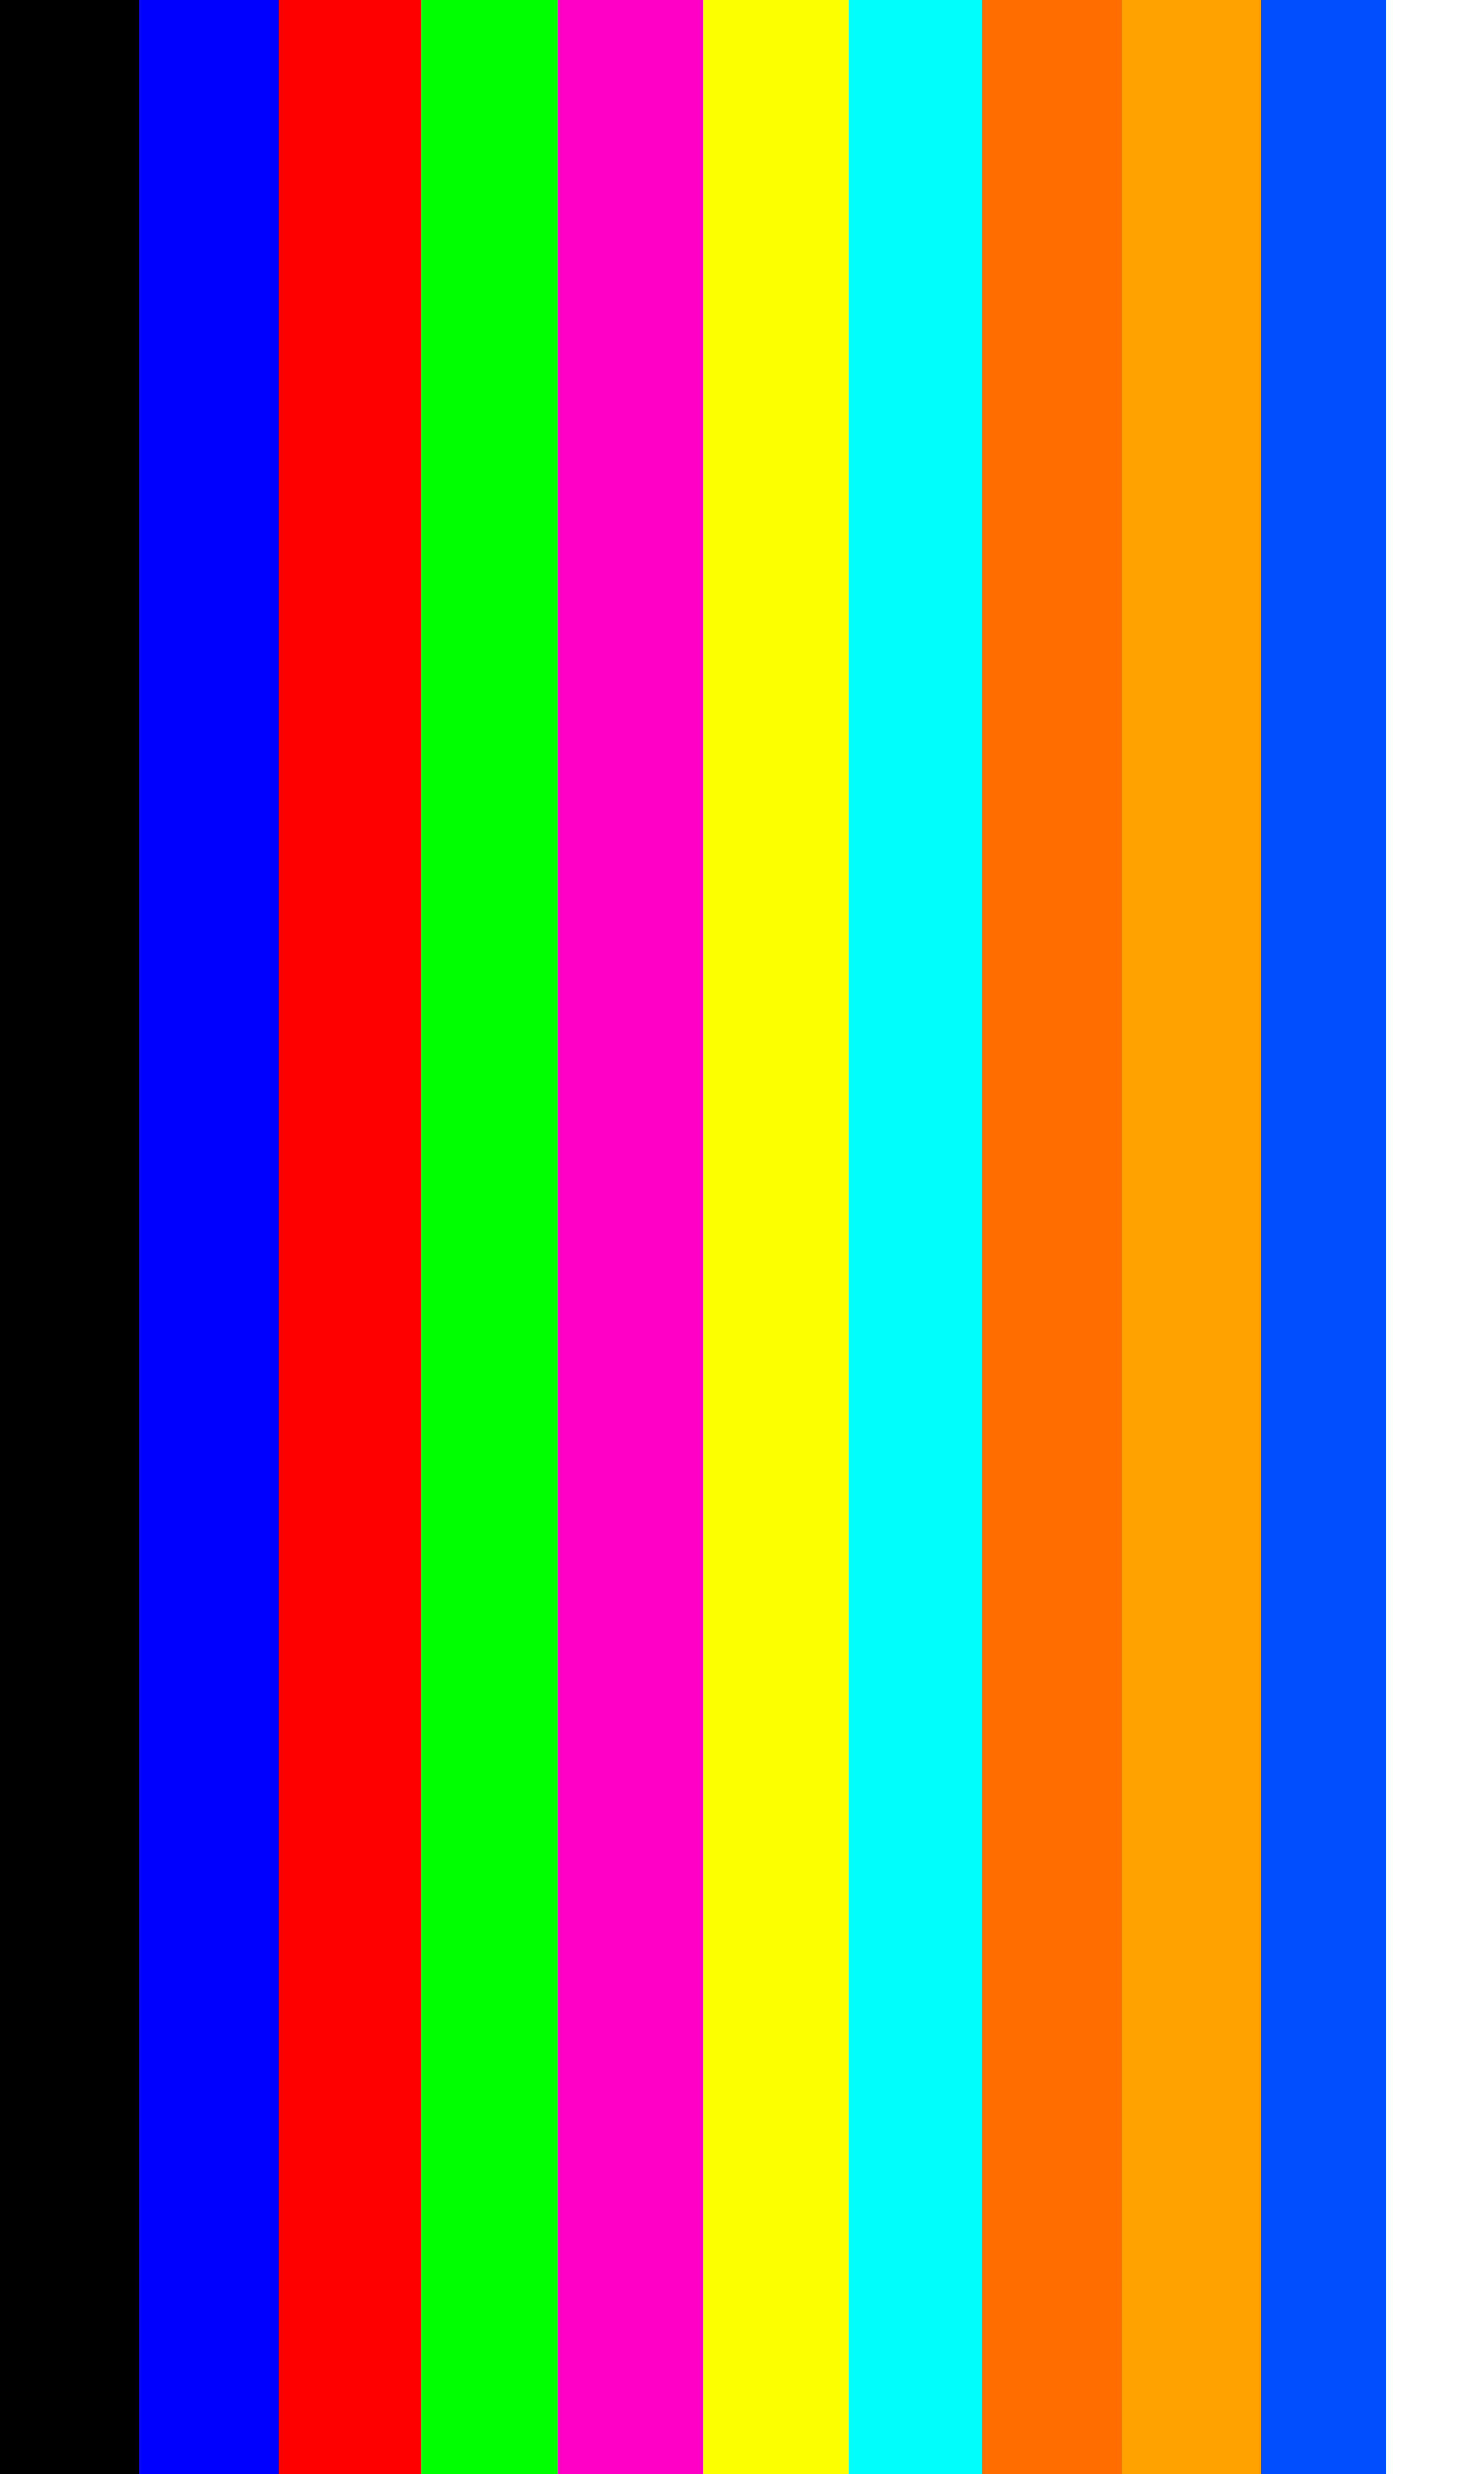
\includegraphics[scale=0.5]{imagenes/colores_demosicing_vecino.png}
    \caption{Vecinos}
    \end{center}
\end{figure}


